%%%%%%%%%%%%%%%%%%%%%%%%%%%%%%%%%%%%%%%%%%%%%%%%%%%%%%%%%%%%%%%%%%%%%%%%%%%%%%%%%%
\begin{frame}[fragile]\frametitle{}
\begin{center}
{\Large Introduction to CAD}
\end{center}
\end{frame}


%%%%%%%%%%%%%%%%%%%%%%%%%%%%%%%%%%%%%%%%%%%%%%%%%%%%%%%%%%%%%%%%%%%%%%%%%%%%%%%%%%
\begin{frame}[fragile]\frametitle{Why CAD?}
\begin{itemize}
\item How to model real world objects? - Design
\item How to put forth ideas in visual manner – Communication
\item How to verify that design serves the purpose – Analysis
\item How to get it made? – Manufacturing
\end{itemize}

All of the above can happen without Computers, but \ldots 

\end{frame}

%%%%%%%%%%%%%%%%%%%%%%%%%%%%%%%%%%%%%%%%%%%%%%%%%%%%%%%%%%%%%%%%%%%%%%%%%%%%%%%%%%
\begin{frame}[fragile]\frametitle{Why CAD?}

Better if assisted by Computers/Software

That's why : Computer Aided $\ldots$ (CAx)
\end{frame}

%%%%%%%%%%%%%%%%%%%%%%%%%%%%%%%%%%%%%%%%%%%%%%%%%%%%%%%%%%%%%%%%%%%%%%%%%%%%%%%%%%
\begin{frame}[fragile]\frametitle{}
\begin{center}
{\Large History}
\end{center}
\end{frame}

%%%%%%%%%%%%%%%%%%%%%%%%%%%%%%%%%%%%%%%%%%%%%%%%%%%%%%%%%%%%%%%%%%%%%%%%%%%%%%%%%%
\begin{frame}[fragile]\frametitle{History}
\begin{itemize}
\item The first source of CAD resulted from attempts to automate the drafting process.
\item These developments were pioneered by the General Motors Research Laboratories in the early 1960s.
\item CAD became more widely used after 1970 because of technological advancements.
\item CAD allowed users to design products much quicker without the production of an actual product.

\end{itemize}

\end{frame}

%%%%%%%%%%%%%%%%%%%%%%%%%%%%%%%%%%%%%%%%%%%%%%%%%%%%%%%%%%%%%%%%%%%%%%%%%%%%%%%%%%
\begin{frame}[fragile]{Evolution of CAD Technology}
\begin{center}
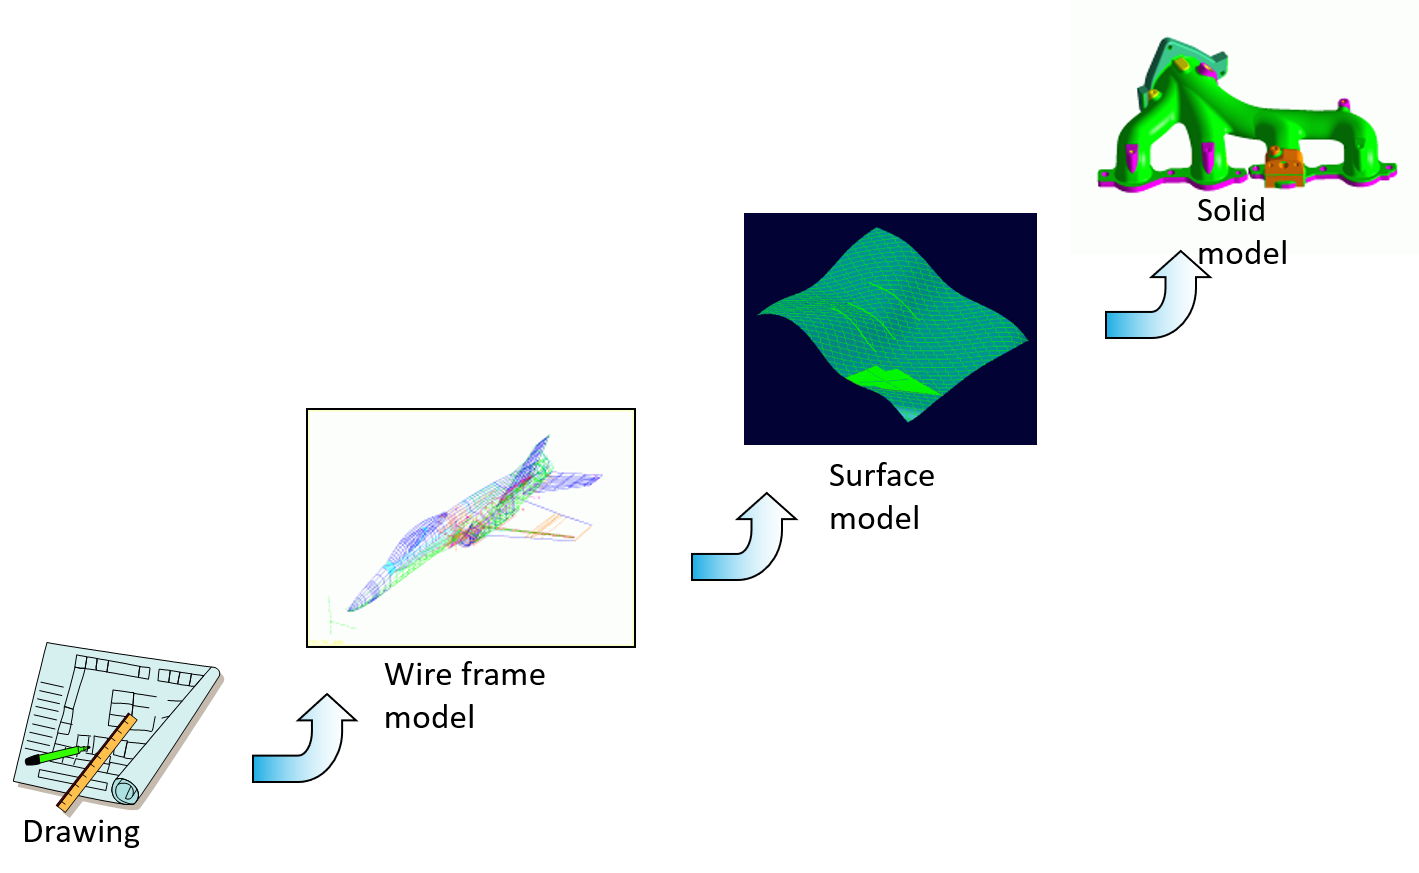
\includegraphics[width=0.9\linewidth,keepaspectratio]{geomod1}
\end{center}
\end{frame}

%%%%%%%%%%%%%%%%%%%%%%%%%%%%%%%%%%%%%%%%%%%%%%%%%%%%%%%%%%%%%%%%%%%%%%%%%%%%%%%%%%
\begin{frame}[fragile]{Manual drafting}
 \begin{columns}
  \begin{column}{0.55\linewidth}
\begin{itemize}
\item 2D representations used to represent 3D objects
\begin{itemize}
\item multi-view drawings
\item pictorials
\end{itemize}
\item Standards and conventions developed so that 3D object could be built from drawings
\item Drawings created manually or using 2D CAD
\item Difficult to visualize, error-prone, time-consuming
\end{itemize}
  \end{column}%
  \begin{column}{0.45\linewidth}
			\begin{center}
			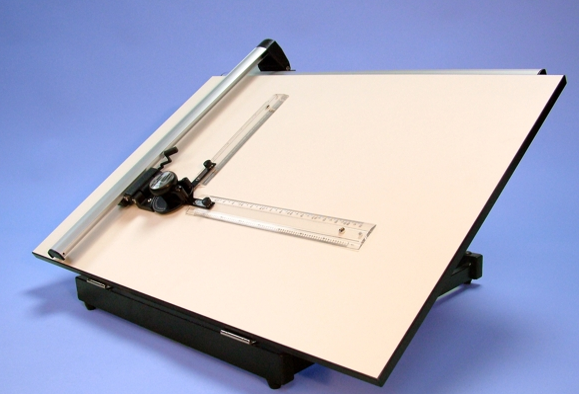
\includegraphics[width=0.9\linewidth,keepaspectratio]{geomod2}
			\end{center}
  \end{column}
 \end{columns}
\end{frame}



%%%%%%%%%%%%%%%%%%%%%%%%%%%%%%%%%%%%%%%%%%%%%%%%%%%%%%%%%%%%%%%%%%%%%%%%%%%%%%%%%%
\begin{frame}[fragile]\frametitle{}
\begin{center}
{\Large Modeling Approaches}
\end{center}
\end{frame}



%%%%%%%%%%%%%%%%%%%%%%%%%%%%%%%%%%%%%%%%%%%%%%%%%%%%%%%%%%%%%%%%%%%%%%%%%%%%%%%%%%
\begin{frame}[fragile]{Modeling Approaches}

\begin{itemize}
\item By dimensionality: 2D/3D
\item 2-Manifold vs Non-manifold
\item Precision: Exact/Approximate
\item What to store?
	\begin{itemize}
	\item Procedure
	\item Result
	\item Hybrid
	\end{itemize}
\end{itemize}
\end{frame}

%%%%%%%%%%%%%%%%%%%%%%%%%%%%%%%%%%%%%%%%%%%%%%%%%%%%%%%%%%%%%%%%%%%%%%%%%%%%%%%%%%
\begin{frame}[fragile]{By dimensionality}
 \begin{columns}
  \begin{column}{0.55\linewidth}
\begin{itemize}
\item 2D model: Point, line, circular arc, planar curve
\item 3D model
	\begin{itemize}
	\item Wire frame

	\item Surface

	\item Solid

	\end{itemize}
\end{itemize}
  \end{column}%
  \begin{column}{0.45\linewidth}
			\begin{center}
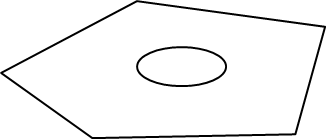
\includegraphics[width=0.5\linewidth,keepaspectratio]{CAD2dprofile.png}
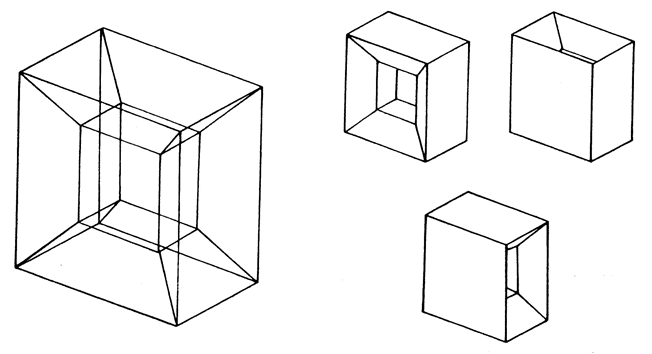
\includegraphics[width=0.6\linewidth,keepaspectratio]{CADWireframe.png}
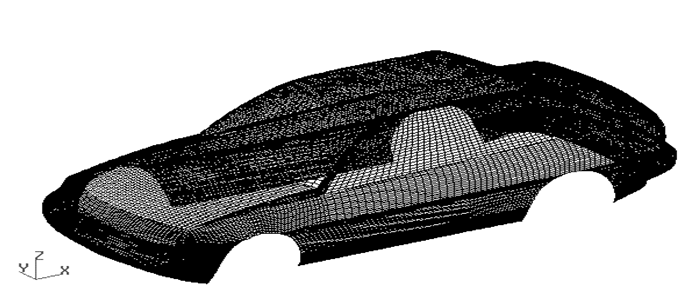
\includegraphics[width=0.6\linewidth,keepaspectratio]{CADSurface.png}
	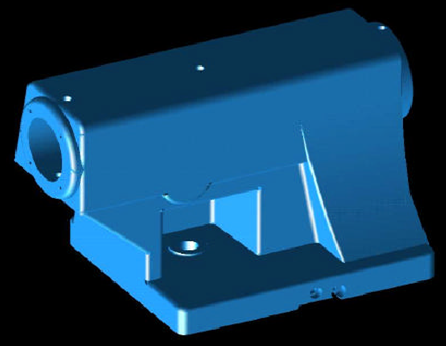
\includegraphics[width=0.6\linewidth,keepaspectratio]{CADSolid.png}

			\end{center}
  \end{column}
 \end{columns}
 
 Advantages and Disadvantages of each?

\end{frame}

%%%%%%%%%%%%%%%%%%%%%%%%%%%%%%%%%%%%%%%%%%%%%%%%%%%%%%%%%%%%%%%%%%%%%%%%%%%%%%%%%%
\begin{frame}[fragile]{2D CAD}
 \begin{columns}
  \begin{column}{0.55\linewidth}
\begin{itemize}
\item Simply replaces manual drawing
\item Provides a set of drawing tools to create 2D elements, like, Lines, circles, arcs, etc.
\item More accurate, easier changes to drawings
\item Still no 3D representation of the object
\item Example: AutoCAD
\end{itemize}
  \end{column}%
  \begin{column}{0.45\linewidth}
			\begin{center}
	
\includegraphics[width=0.9\linewidth,keepaspectratio]{geomod3.png}

			\end{center}
  \end{column}
 \end{columns}
 
\end{frame}

%%%%%%%%%%%%%%%%%%%%%%%%%%%%%%%%%%%%%%%%%%%%%%%%%%%%%%%%%%%%%%%%%%%%%%%%%%%%%%%%%%
\begin{frame}[fragile]\frametitle{2D Applications}
\begin{itemize}
\item Drafting – sketches, architectures, Drawings
\item Art - Sketches, painting
\item Electronic layouts, circuit design
\end{itemize}

			\begin{center}
	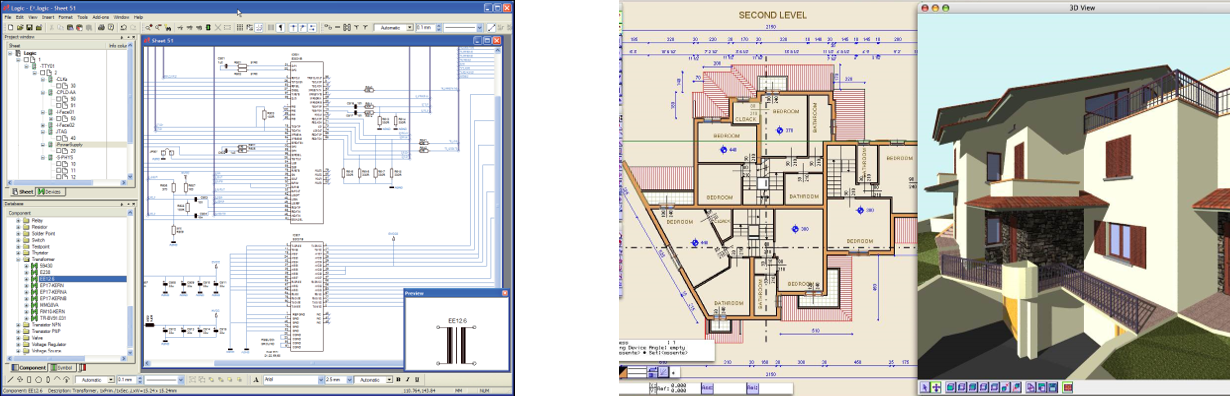
\includegraphics[width=0.7\linewidth,keepaspectratio]{geomod10}
			\end{center}
\end{frame}


%%%%%%%%%%%%%%%%%%%%%%%%%%%%%%%%%%%%%%%%%%%%%%%%%%%%%%%%%%%%%%%%%%%%%%%%%%%%%%%%%%
\begin{frame}[fragile]{3D Wire frame Modeling}
 \begin{columns}
  \begin{column}{0.55\linewidth}
\begin{itemize}
\item Geometric entities are lines and curves in 3D
\item Volume or surfaces of object not defined
\item Easy to store and display
\item Hard to interpret - ambiguous
\end{itemize}
  \end{column}%
  \begin{column}{0.45\linewidth}
			\begin{center}
	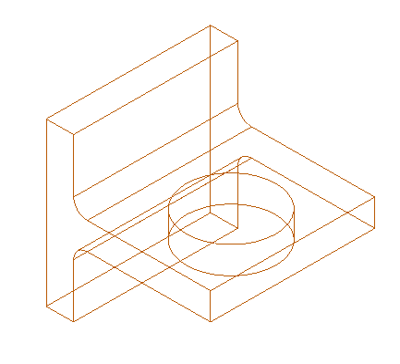
\includegraphics[width=0.9\linewidth,keepaspectratio]{geomod4.png}

			\end{center}
  \end{column}
 \end{columns}
 
\end{frame}

%%%%%%%%%%%%%%%%%%%%%%%%%%%%%%%%%%%%%%%%%%%%%%%%%%%%%%%%%%%%%%%%%%%%%%%%%%%%%%%%%%
\begin{frame}[fragile]{Problems with wire frame models}
			\begin{center}
	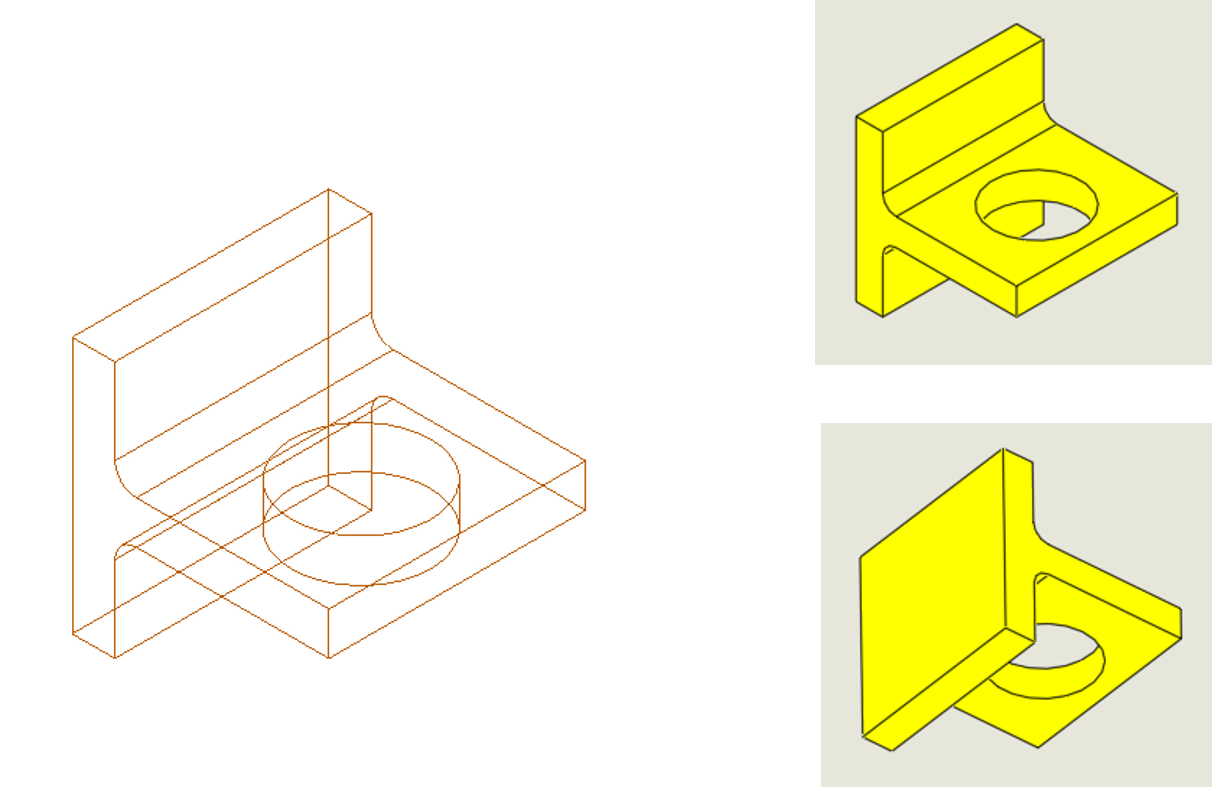
\includegraphics[width=0.9\linewidth,keepaspectratio]{geomod5}
			\end{center}
\end{frame}

%%%%%%%%%%%%%%%%%%%%%%%%%%%%%%%%%%%%%%%%%%%%%%%%%%%%%%%%%%%%%%%%%%%%%%%%%%%%%%%%%%
\begin{frame}[fragile]{Surface Modeling}
			\begin{center}
	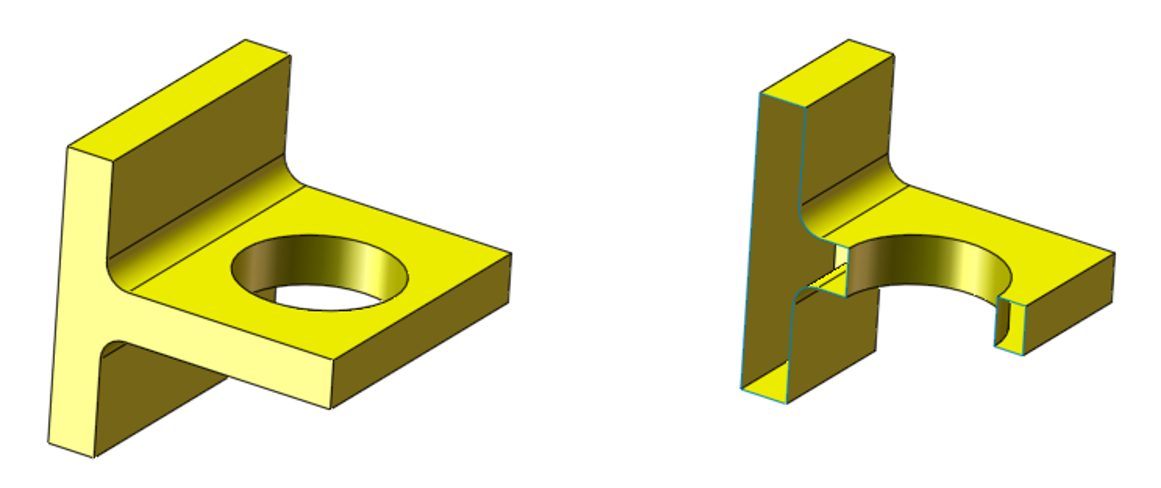
\includegraphics[width=0.9\linewidth,keepaspectratio]{geomod6}
			\end{center}
\end{frame}

%%%%%%%%%%%%%%%%%%%%%%%%%%%%%%%%%%%%%%%%%%%%%%%%%%%%%%%%%%%%%%%%%%%%%%%%%%%%%%%%%%
\begin{frame}[fragile]{3D Surface Modeling}
 \begin{columns}
  \begin{column}{0.55\linewidth}
\begin{itemize}
\item Models 2D surfaces in 3D space
\item All points on surface are defined, useful for machining, visualization, etc.
\item Surfaces have no thickness, objects have no volume or solid properties
\item Surfaces may be open
\end{itemize}
  \end{column}%
  \begin{column}{0.45\linewidth}
			\begin{center}
	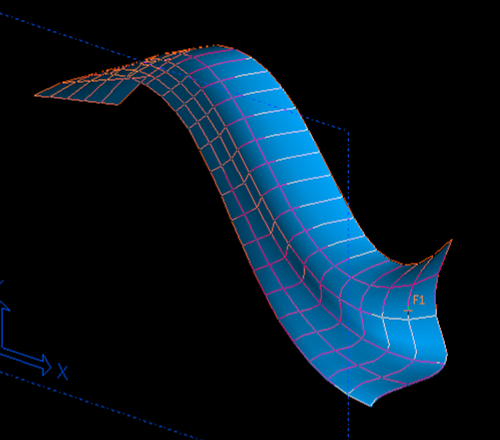
\includegraphics[width=0.9\linewidth,keepaspectratio]{geomod7}

			\end{center}
  \end{column}
 \end{columns}
 
\end{frame}

%%%%%%%%%%%%%%%%%%%%%%%%%%%%%%%%%%%%%%%%%%%%%%%%%%%%%%%%%%%%%%%%%%%%%%%%%%%%%%%%%%
\begin{frame}[fragile]{Surface Modeling}
A Surface Model created using Alias Studio Tools

			\begin{center}
	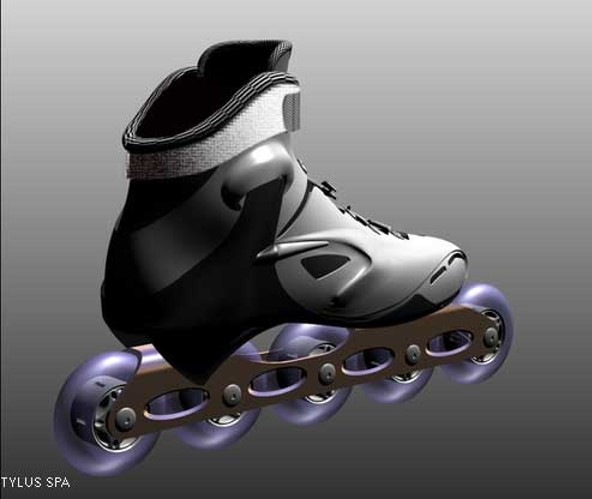
\includegraphics[width=0.7\linewidth,keepaspectratio]{geomod8}
			\end{center}
\end{frame}

%%%%%%%%%%%%%%%%%%%%%%%%%%%%%%%%%%%%%%%%%%%%%%%%%%%%%%%%%%%%%%%%%%%%%%%%%%%%%%%%%%
\begin{frame}[fragile]{Surface Modeling}
Surface Model created using Rhino

			\begin{center}
	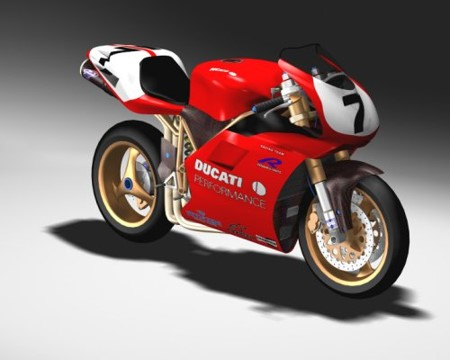
\includegraphics[width=0.7\linewidth,keepaspectratio]{geomod9}
			\end{center}
\end{frame}


%%%%%%%%%%%%%%%%%%%%%%%%%%%%%%%%%%%%%%%%%%%%%%%%%%%%%%%%%%%%%%%%%%%%%%%%%%%%%%%%%%
\begin{frame}[fragile]\frametitle{Why draw 3D Models?}
\begin{itemize}
\item 3D models are easier to interpret.
\item Less expensive than building a physical model.
\item 3D models can be altered easily, create more concepts.
\item 3D models can be used to perform engineering analysis, finite element analysis (stress, deflection, thermal…..) and motion analysis.
\item 3D models can be used directly in manufacturing, Computer Numerical Control (CNC).
\end{itemize}

\end{frame}

%%%%%%%%%%%%%%%%%%%%%%%%%%%%%%%%%%%%%%%%%%%%%%%%%%%%%%%%%%%%%%%%%%%%%%%%%%%%%%%%%%
\begin{frame}[fragile]{Solid, parametric, feature based modeling}
 \begin{columns}
  \begin{column}{0.55\linewidth}
\begin{itemize}
\item Complete and unambiguous
\item Solid - models have volume, and mass properties
\item Feature based - geometry built up by adding and subtracting features
\item Parametric - geometry can be modified by changing dimensions
\end{itemize}
  \end{column}%
  \begin{column}{0.45\linewidth}
			\begin{center}
	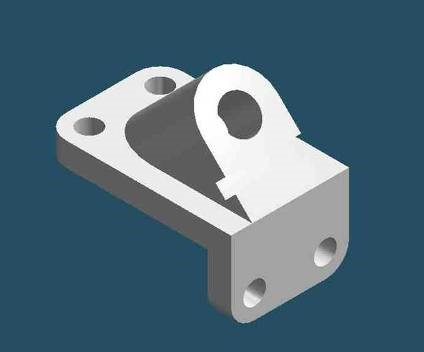
\includegraphics[width=0.9\linewidth,keepaspectratio]{geomod14}

			\end{center}
  \end{column}
 \end{columns}
 
\end{frame}




%%%%%%%%%%%%%%%%%%%%%%%%%%%%%%%%%%%%%%%%%%%%%%%%%%%%%%%%%%%%%%%%%%%%%%%%%%%%%%%%%%
\begin{frame}[fragile]\frametitle{3D Applications}
\begin{itemize}
\item CAD (Computer Aided Design)
\item CAM (Computer Aided Manufacturing)
\item CAE (Computer Aided Engineering) Finite Element Method
\item CG (Computer Graphics)
\end{itemize}

			\begin{center}
	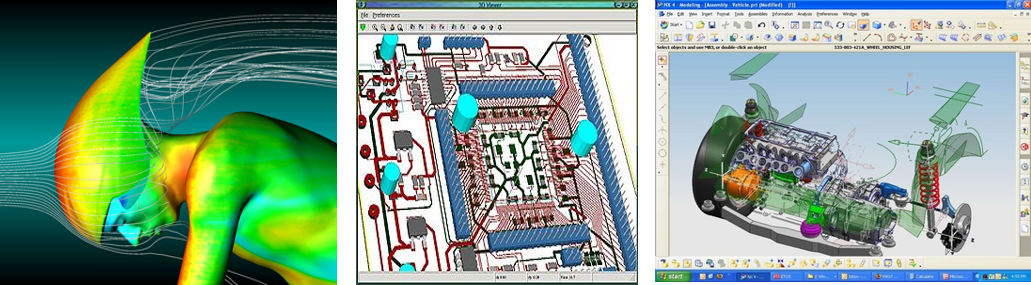
\includegraphics[width=0.9\linewidth,keepaspectratio]{geomod11}
			\end{center}
\end{frame}

%%%%%%%%%%%%%%%%%%%%%%%%%%%%%%%%%%%%%%%%%%%%%%%%%%%%%%%%%%%%%%%%%%%%%%%%%%%%%%%%%%
\begin{frame}[fragile]\frametitle{Basics of Finite Element Analysis (FEA) }
\begin{itemize}
\item A complex problem is divided into a smaller and simpler problems that can be solved by using the existing knowledge of mechanics of materials and mathematical tools 
\item Modern mechanical design involves complicated shapes, sometimes made of different materials that as a whole cannot be solved by existing mathematical tools. Engineers need the FEA to evaluate their designs

\end{itemize}

			\begin{center}
	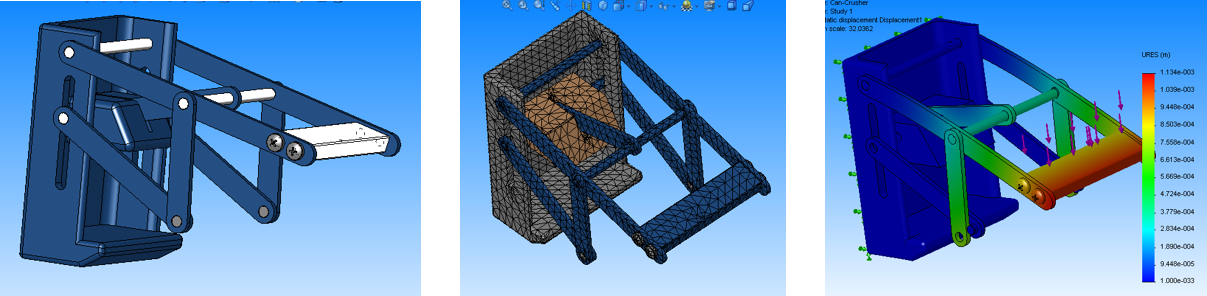
\includegraphics[width=0.7\linewidth,keepaspectratio]{geomod12}
			\end{center}
\end{frame}

%%%%%%%%%%%%%%%%%%%%%%%%%%%%%%%%%%%%%%%%%%%%%%%%%%%%%%%%%%%%%%%%%%%%%%%%%%%%%%%%%%
\begin{frame}[fragile]\frametitle{Computer Numerical Control (CNC)}
A CNC machine is an NC machine with the added feature of an on-board computer.

			\begin{center}
	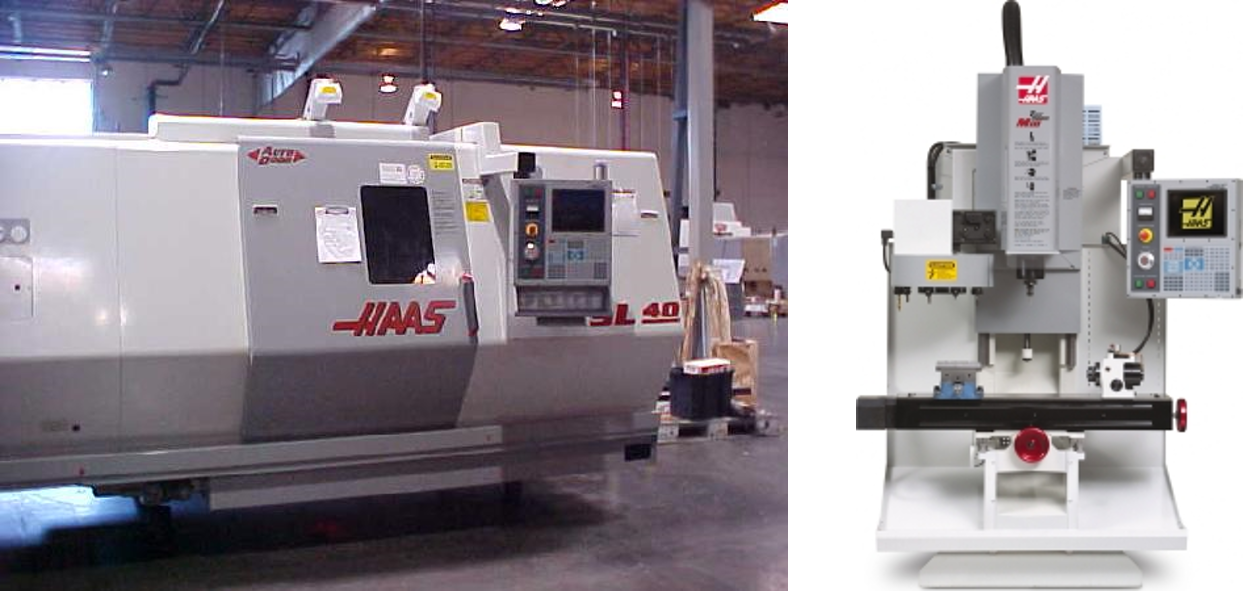
\includegraphics[width=0.7\linewidth,keepaspectratio]{geomod13}
			\end{center}
\end{frame}

%%%%%%%%%%%%%%%%%%%%%%%%%%%%%%%%%%%%%%%%%%%%%%%%%%%%%%%%%%%%%%%%%%%%%%%%%%%%%%%%%%
\begin{frame}[fragile]\frametitle{}
\begin{center}
{\Large Solids}
\end{center}
\end{frame}

%%%%%%%%%%%%%%%%%%%%%%%%%%%%%%%%%%%%%%%%%%%%%%%%%%%%%%%%%%%%%%%%%%%%%%%%%%%%%%%%%%
\begin{frame}[fragile]\frametitle{What is a Solid?}
\begin{itemize}
\item Define Solid?
\item How would you represent Solid in software (data model)?
\end{itemize}
\end{frame}

%%%%%%%%%%%%%%%%%%%%%%%%%%%%%%%%%%%%%%%%%%%%%%%%%%%%%%%%%%%%%%%%%%%%%%%%%%%%%%%%%%
\begin{frame}[fragile]\frametitle{Cloud of points }
\begin{itemize}
\item The simplest form
\item Unorganized / organized points
\item Too many points to represent the desired shape
\item Hard to handle $\rightarrow$ further processing is required
\item Obtained by digitizing
\begin{itemize}
\item CMM (coordinate measuring machine)
\item Laser range scanner
\item \ldots
\end{itemize}
\end{itemize}

			\begin{center}
	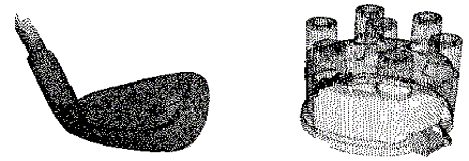
\includegraphics[width=0.7\linewidth,keepaspectratio]{geomod15}
			\end{center}
\end{frame}

%%%%%%%%%%%%%%%%%%%%%%%%%%%%%%%%%%%%%%%%%%%%%%%%%%%%%%%%%%%%%%%%%%%%%%%%%%%%%%%%%%
\begin{frame}[fragile]\frametitle{Mesh}
\begin{itemize}
\item Most popular approximation model
\item Graphics, RP, CAD/CAM, DMU, CAE
\item Hard to handle
\item Triangular mesh, Quad mesh, General polygonal mesh
\item Create mesh by
\begin{itemize}
\item triangulating cloud of points
\item faceting exact surface model
\end{itemize}
\item Example: 123D Catch
\end{itemize}

			\begin{center}
	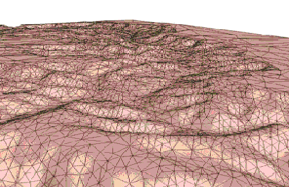
\includegraphics[width=0.6\linewidth,keepaspectratio]{geomod16}
			\end{center}
\end{frame}


%%%%%%%%%%%%%%%%%%%%%%%%%%%%%%%%%%%%%%%%%%%%%%%%%%%%%%%%%%%%%%%%%%%%%%%%%%%%%%%%%%
\begin{frame}[fragile]{So, Classification By Precision}
 \begin{columns}
  \begin{column}{0.55\linewidth}
\begin{itemize}
\item Exact (?) model : Continuous/Smooth representation. Explicit / implicit / parametric curves / surfaces
\item Approximate model
	\begin{itemize}
	\item Cloud of points 

	\item Voxel

	\item Mesh

	\end{itemize}
\end{itemize}
  \end{column}%
  \begin{column}{0.45\linewidth}
			\begin{center}
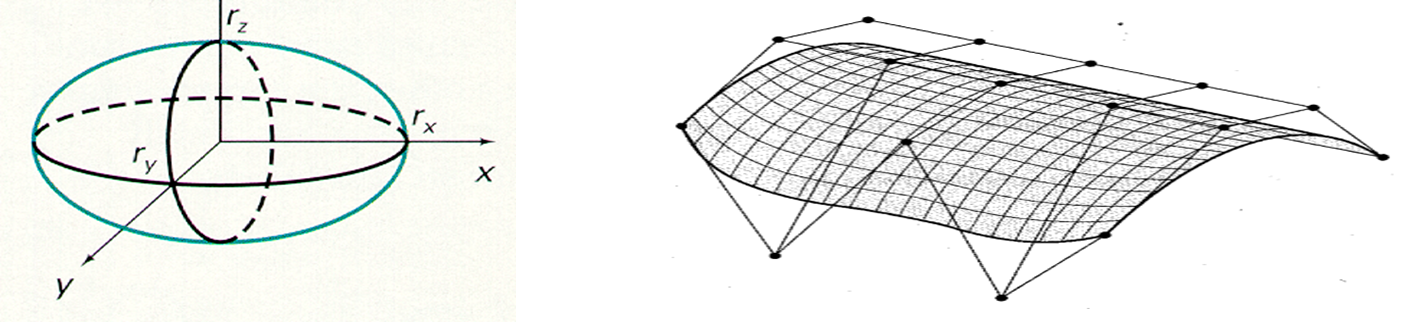
\includegraphics[width=0.5\linewidth,keepaspectratio]{images/CADExact.png}
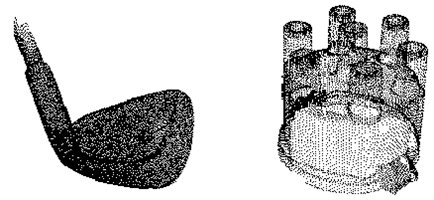
\includegraphics[width=0.6\linewidth,keepaspectratio]{images/CADCloud.png}
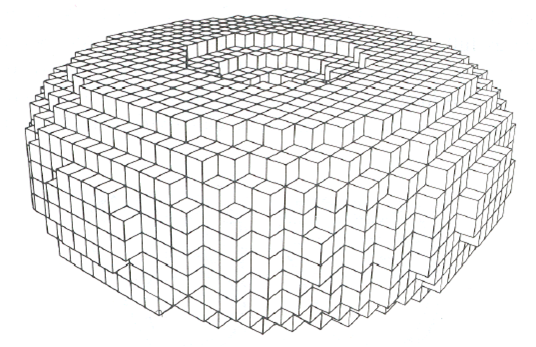
\includegraphics[width=0.6\linewidth,keepaspectratio]{images/CADVoxel.png}
	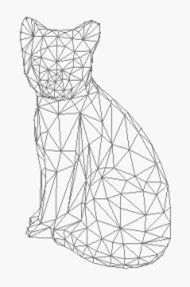
\includegraphics[width=0.6\linewidth,keepaspectratio]{images/CADMesh.png}

			\end{center}
  \end{column}
 \end{columns}
\end{frame}



%%%%%%%%%%%%%%%%%%%%%%%%%%%%%%%%%%%%%%%%%%%%%%%%%%%%%%%%%%%%%%%%%%%%%%%%%%%%%%%%%%
\begin{frame}[fragile]{By Storage}
\begin{itemize}
\item Procedural model : CSG (Constructive Solid Geometry)

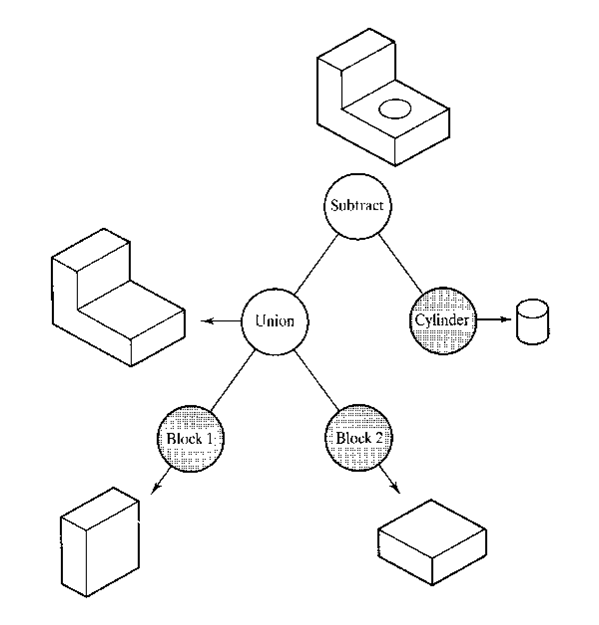
\includegraphics[width=0.4\linewidth,keepaspectratio]{images/CADCSG.png}
\item Result based model : B-Rep (Boundary representation)

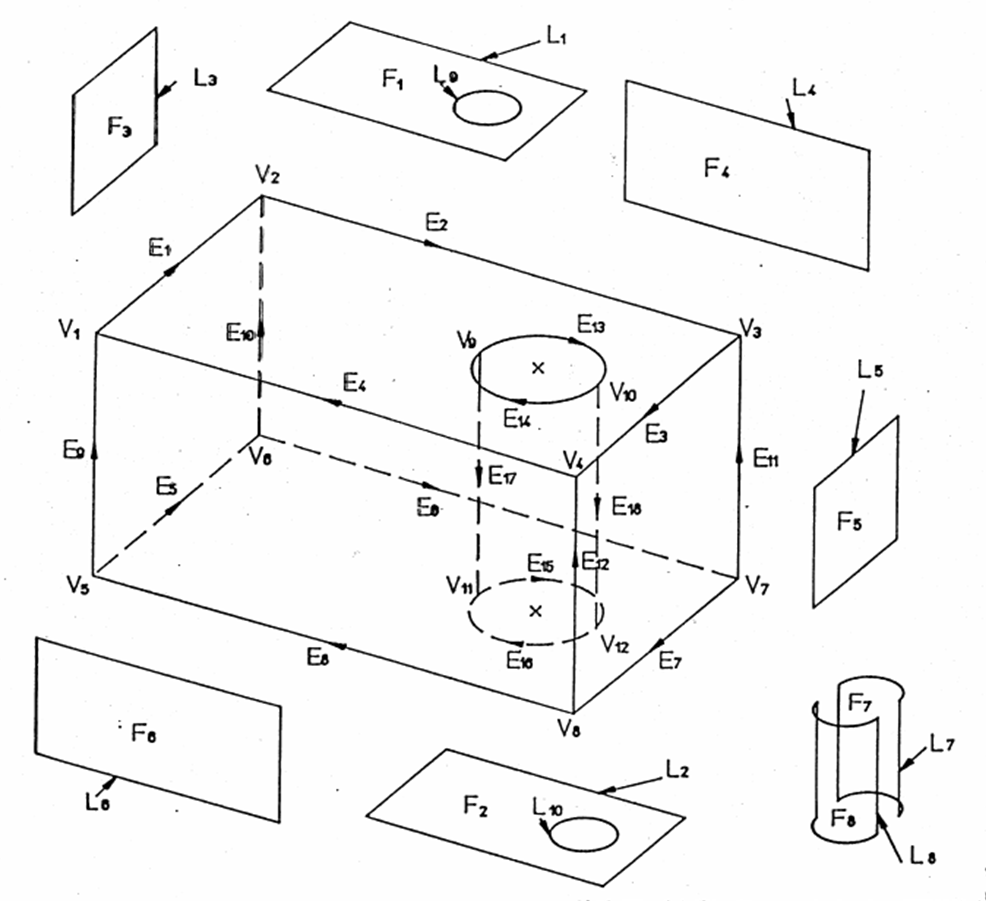
\includegraphics[width=0.4\linewidth,keepaspectratio]{images/CADBrep.png}
\end{itemize}
\end{frame}

%%%%%%%%%%%%%%%%%%%%%%%%%%%%%%%%%%%%%%%%%%%%%%%%%%%%%%%%%%%%%%%%%%%%%%%%%%%%%%%%%%
\begin{frame}[fragile]{B-Rep model}
 \begin{columns}
  \begin{column}{0.55\linewidth}
	Topological element
	\begin{itemize}
	\item Vertex
	\item Edge
	\item Loop (Edge list)
	\item Face
	\item Lump
	\item Body
	\end{itemize}
	
  \end{column}%
  \begin{column}{0.45\linewidth}
	Geometrical element

	\begin{itemize}
	\item Point
	\item Curve
	\item Composite curve
	\item Surface, trimmed surface
	\item N/A
	\item N/A
	\end{itemize}
  \end{column}
 \end{columns}
\end{frame}

%%%%%%%%%%%%%%%%%%%%%%%%%%%%%%%%%%%%%%%%%%%%%%%%%%%%%%%%%%%%%%%%%%%%%%%%%%%%%%%%%%
\begin{frame}[fragile]\frametitle{Euler-Poincare formula}
\begin{itemize}
\item For a polyhedron $ V - E + F - 2 = 0$               
\begin{itemize}
\item V = Vertices
\item E = Edges
\item F = Faces
\end{itemize}
\item Example: A tetrahedron has four vertices, four faces, and six edges
$4-6+4=2$
\end{itemize}
\end{frame}

%%%%%%%%%%%%%%%%%%%%%%%%%%%%%%%%%%%%%%%%%%%%%%%%%%%%%%%%%%%%%%%%%%%%%%%%%%%%%%%%%%
\begin{frame}[fragile]\frametitle{Extension to Euler-Poincare formula}
\begin{itemize}
\item A solid can have holes 
\item A face may have a loop or ring of vertices `floating‘, i.e. unconnected by edges to the other vertices of the face 
\end{itemize}
\end{frame}


%%%%%%%%%%%%%%%%%%%%%%%%%%%%%%%%%%%%%%%%%%%%%%%%%%%%%%%%%%%%%%%%%%%%%%%%%%%%%%%%%%
\begin{frame}[fragile]\frametitle{Extension to Euler-Poincare formula}
$V-E+F-H=2(C-G)$

\begin{itemize}
\item V = Vertices
\item E = Edges
\item F = Faces
\item H = Holes in faces  
\item C = Components (or shells)
\item G = Genus (holes through solid)
\end{itemize}

``Tweaking'' (deformations, twisting, and stretching but not tearing, or cutting ) solids modifies the solid without changing the topology or the above numbers.

\end{frame}

%%%%%%%%%%%%%%%%%%%%%%%%%%%%%%%%%%%%%%%%%%%%%%%%%%%%%%%%%%%%%%%%%%%%%%%%%%%%%%%%%%
\begin{frame}[fragile]\frametitle{A solid with holes and loops }

\begin{itemize}
\item $V-E+F-H=2(C-G)$
\item $24 – 36 + 15 – 3 = 2( 1 – 1)$
\end{itemize}

			\begin{center}
	
\includegraphics[width=0.6\linewidth,keepaspectratio]{geomod17}
			\end{center}
\end{frame}


%%%%%%%%%%%%%%%%%%%%%%%%%%%%%%%%%%%%%%%%%%%%%%%%%%%%%%%%%%%%%%%%%%%%%%%%%%%%%%%%%%
\begin{frame}[fragile]\frametitle{Limitations}

\begin{itemize}
\item Necessary but not sufficient condition for a valid representation.
\item Example: 8 vertices, 12 edges, 6 faces
\end{itemize}

			\begin{center}
	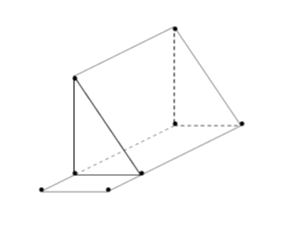
\includegraphics[width=0.6\linewidth,keepaspectratio]{geomod18}
			\end{center}
\end{frame}

%%%%%%%%%%%%%%%%%%%%%%%%%%%%%%%%%%%%%%%%%%%%%%%%%%%%%%%%%%%%%%%%%%%%%%%%%%%%%%%%%%
\begin{frame}[fragile]\frametitle{Brep vs Mesh  }

The object is represented by subdivision/discretization such as mesh and other geometric primitives.


			\begin{center}
	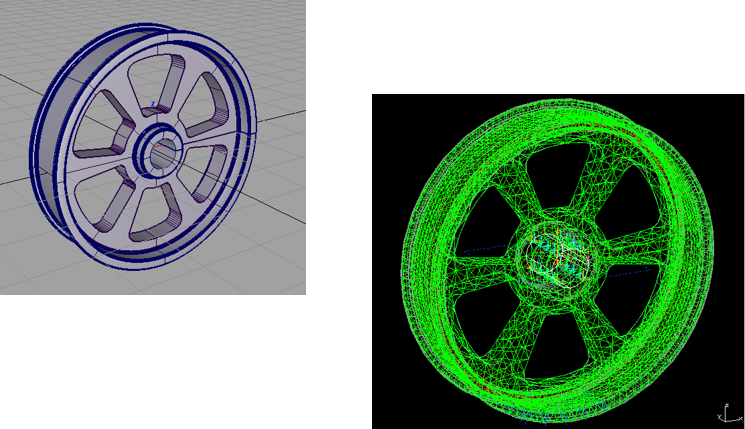
\includegraphics[width=0.9\linewidth,keepaspectratio]{geomod19}
			\end{center}
\end{frame}

%%%%%%%%%%%%%%%%%%%%%%%%%%%%%%%%%%%%%%%%%%%%%%%%%%%%%%%%%%%%%%%%%%%%%%%%%%%%%%%%%%
\begin{frame}[fragile]\frametitle{Parametric, Feature-based Solid Model}
			\begin{center}
	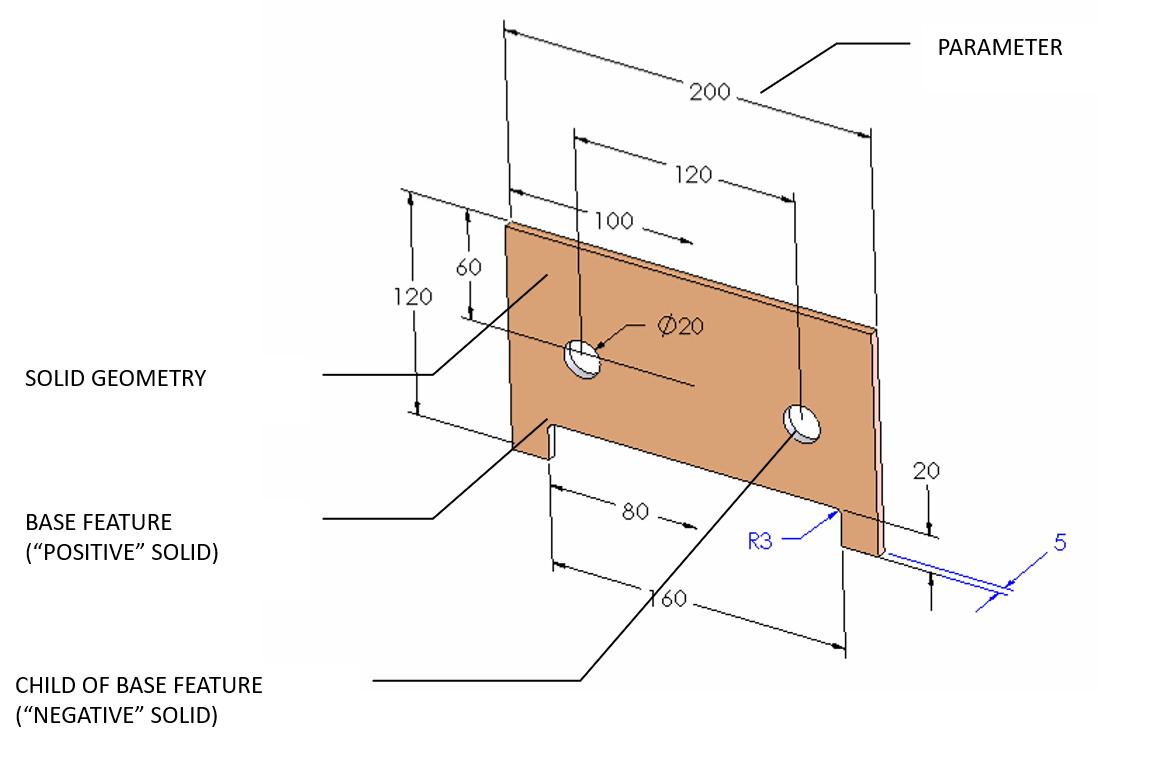
\includegraphics[width=0.9\linewidth,keepaspectratio]{geomod20}
			\end{center}
\end{frame}

%%%%%%%%%%%%%%%%%%%%%%%%%%%%%%%%%%%%%%%%%%%%%%%%%%%%%%%%%%%%%%%%%%%%%%%%%%%%%%%%%%
\begin{frame}[fragile]\frametitle{Solid, parametric, feature-based Modeling Software}

\begin{itemize}
\item High-end (more powerful)
\begin{itemize}

\item NX (UGS)
\item Catia (Dassault Systémes)
\item Pro/Engineer (Parametric Technologies Corp.)
\end{itemize}

\item Mid-Range (easier to use)
\begin{itemize}

\item Solid Edge (UGS)
\item Inventor (Autodesk)
\item SolidWorks (SolidWorks Corp.)
\end{itemize}
\end{itemize}

They all work basically the same way, $somewhat$!!

\end{frame}